\documentclass{article} % For LaTeX2e
\usepackage{nips13submit_e,times}
\usepackage{hyperref}
\usepackage{url}
\usepackage{graphicx}
\usepackage{caption}
\usepackage{subcaption}
%\documentstyle[nips13submit_09,times,art10]{article} % For LaTeX 2.09

\usepackage{amsmath}
\usepackage{algorithm}
\usepackage{algpseudocode}

\title{House Prices Prediction using Machine Learning}


\author{
Gang Wu\\
\texttt{gangwu@stanford.edu} \\
}

% The \author macro works with any number of authors. There are two commands
% used to separate the names and addresses of multiple authors: \And and \AND.
%
% Using \And between authors leaves it to \LaTeX{} to determine where to break
% the lines. Using \AND forces a linebreak at that point. So, if \LaTeX{}
% puts 3 of 4 authors names on the first line, and the last on the second
% line, try using \AND instead of \And before the third author name.

\newcommand{\fix}{\marginpar{FIX}}
\newcommand{\new}{\marginpar{NEW}}

\nipsfinalcopy % Uncomment for camera-ready version

\begin{document}


\maketitle

\section{Introduction}

Real estate always been a hot topic, especially in the recent years.
In this project, I work on a practical problem on this topic:
given a set of features (e.g. location, build year, etc.) for a house,
how much will it sell?
The answer to this question will attract great interest to house buyers and sellers.
I will explore various machine learning techniques in this project to help answer this question.

\section{Problem Definition}

\subsection{Input \& Output}

The input to my problem would be a set of feature values for a house,
such as `year built', `lot size', `living room size', `school district', etc.
The output is the predicted sale price.

As a concrete example, below is a simplified set of feature values for a house as an input:

$['year\_built', 'lot\_size', 'livingroom\_size', 'school\_score'] = [2001, 3000, 800, 9]$

The output would be its sale price in USD: $650000$.

\subsection{Evaluation Metric}

For this work, I use Root-Mean-Squared-Error (RMSE) to evaluate the model \cite{rmse}:
\begin{equation*}
	RMSE = \sqrt{\frac{\sum_{t=1}^{T}(y_t' - y_t)}{T}}
\end{equation*}

Here, $y_t'$ denotes the logarithm of predicted house price 
and $y_t$ denotes the logarithm of real house price.
Taking logs will help make sure that errors in predicting expensive houses 
and cheap houses affect the result equally.

\section{Baseline Implementation}

\subsection{Data}

The baseline dataset I used is `Ames Housing dataset' obtained from Kaggle \cite{kaggle}.
This dataset is small (1461 houses each with 81 features on the training set)
and out of date. 
I use it only for initial implementation of different ML algorithms
and building up a baseline framework.
For the next step of this project,
a web crawler will be built to obtain more data
from online real estate websites.
 
\subsection{Exploratory Data Analysis}

Some exploratory analysis on the `Ames Housing dataset' is shown in Figure 1.
From the distribution of the sale price,
we can see most of the houses are in 129K to 214K range.
Figure 1 (b) shows the living room area v.s. sale price,
which roughly have a linear relationship.
Figure 1 (c) shows the overall quality v.s. sale price.
It shows the overall quality is a very strong indicator of the sale price.

\begin{figure}[h]
	\begin{center}
		%\fbox{\rule{0pt}{2in} \rule{0.9\linewidth}{0pt}}
		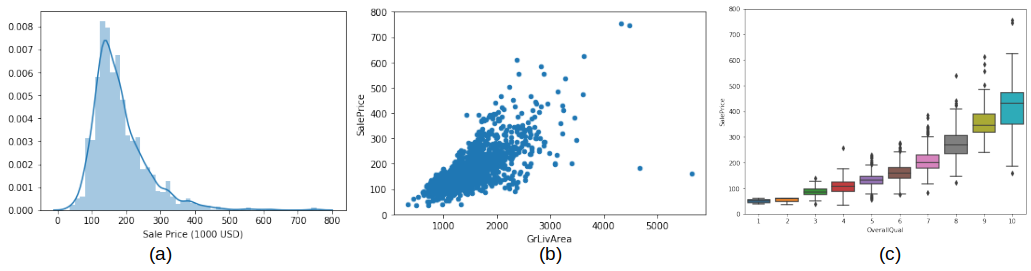
\includegraphics[width=1\linewidth]{fig/eda.png}
	\end{center}
	\caption{(a) sale price distribution. (b) living room area v.s. sale price (1000 USD). (c) overall quality v.s. sale price (1000 USD).}
	\label{fig:long}
	\label{fig:onecol}
\end{figure}

Top 6 correlated features with sale price is shown in the table below:

\begin{table*}[h]
	\begin{center}
		\begin{tabular}{|l|cccccc|}
			\hline
			Feature Name: &
			OverallQual &
			GrLivArea &
			GarageArea &
			TotalBsmtSF &
			1stFlrSF &
			FullBath \\
			\hline
			Correlation: &
			0.81 &
			0.70 &
			0.65 &
			0.61 &
			0.59 &
			0.59 \\
			\hline
		\end{tabular}
	\end{center}
	\caption{Most important features correlating with sales price.}
\end{table*}

\subsection{Preprocessing}

The dataset is splited into two parts: 70\% on the $training\_set$ for training
and 30\% on the $dev\_set$ for cross validation.
I also extracted all the 37 numerical features while ignoring the
rest 43 categorical features for a simple baseline implementation.
The missing feature values are filled using the median value of the feature.
This ends up with the $training\_set$ dimension $(1022, 37)$ and $dev\_set$ dimension $(438, 37)$.

\subsection{Models \& Experimental Results}

Figure 2 (a) shows the linear regression results \cite{lr} on $training\_set$ and $dev\_set$
and Figure 2 (b) shows the results of XGBoost\cite{xgboost}.
The corresponding RMSE value is shown in Table 2.
From the result, we can see the XGBoost model helps remove the few outliers
and also significantly improved the results on the $dev\_set$.

\begin{figure}[h]
	\begin{center}
		%\fbox{\rule{0pt}{2in} \rule{0.9\linewidth}{0pt}}
		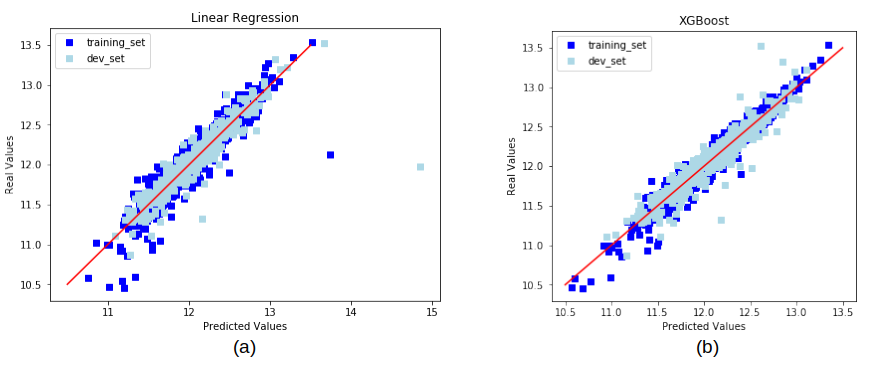
\includegraphics[width=1\linewidth]{fig/exp.png}
	\end{center}
	\caption{(a) Linear regression. (b) XGBoost.}
	\label{fig:long}
	\label{fig:onecol}
\end{figure}

\begin{table*}[h]
	\begin{center}
		\begin{tabular}{|l|cc|}
			\hline
			RMSE &
			TrainSet &
			DevSet \\
			\hline
			LR & 0.142 & 0.184 \\
			\hline
			XGB & 0.136 & 0.148 \\
			\hline
		\end{tabular}
	\end{center}
	\caption{RMSE with linear regression and XGBoost.}
\end{table*}

\subsection{Next Step}

The next step of this project is to obtain more data from the real estate websites.
Also, more feature engineering work and machine learning models need to be implemented and tuned.

{\small
	%\bibliographystyle{ieee}
	\bibliographystyle{unsrt}
	\bibliography{nips2013}
}



\end{document}
